\section{Minimum power SRP PHAT using a microphone array}
\subsection{Microphone array geometry}

\subsubsection{Effect of angular resolution of localization}
Similar to the 2D angular resolution due to a single pair (Fig. \ref{fig:res_diff}), the tetrahedral array has its own 3D  angular resolution depending on the sample rate and the array aperture size. Fig. \ref{fig:res_diff_3d} describes the angular resolution of a tetrahedral array of aperture 1m for different sample rates. If the SRP search space is $360\degree$ by $180\degree$, and the resolution of search is $1\degree$, there will be some angular locations where the delay in sample between a microphone pair is fractional. For simplicity, this fractional delay is rounded for all plots in this thesis. This means that certain locations will contain duplicate data from the nearest integral delay location to themselves. Obviously, the resolution improves for higher sample rate.
\begin{figure}[H]
    \centering
    \begin{subfigure}[b]{0.96\textwidth}
    \centering
    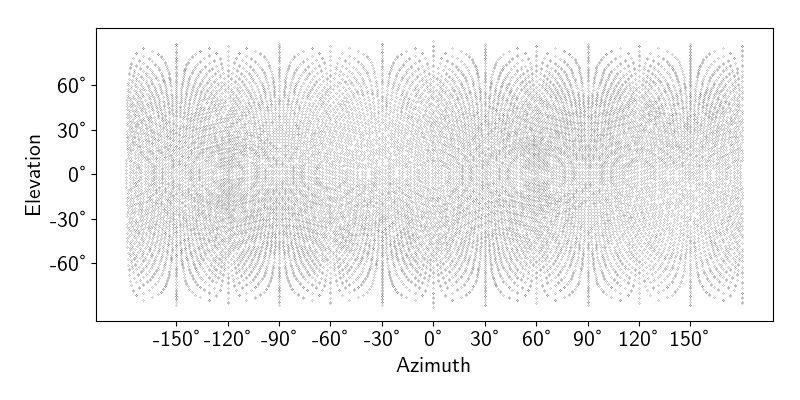
\includegraphics[width=0.7\textwidth]{Figures/res3d12k.png}
\end{subfigure}
\vskip \baselineskip
\begin{subfigure}[b]{0.96\textwidth}
    \centering
    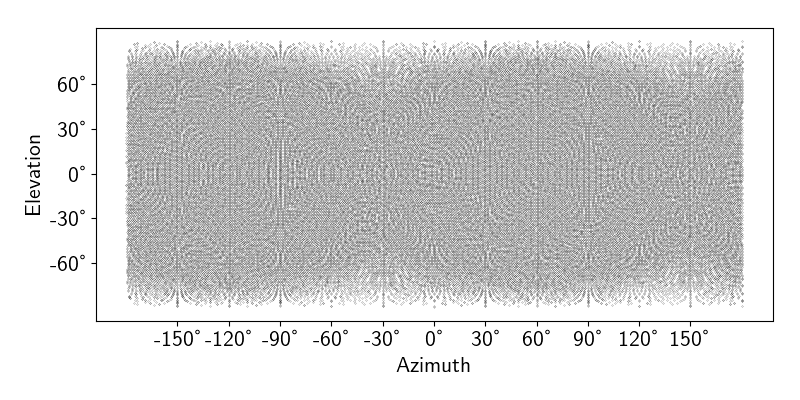
\includegraphics[width=0.7\textwidth]{Figures/res3d48k.png}
\end{subfigure}
\vskip \baselineskip
\begin{subfigure}[b]{0.96\textwidth}
    \centering
    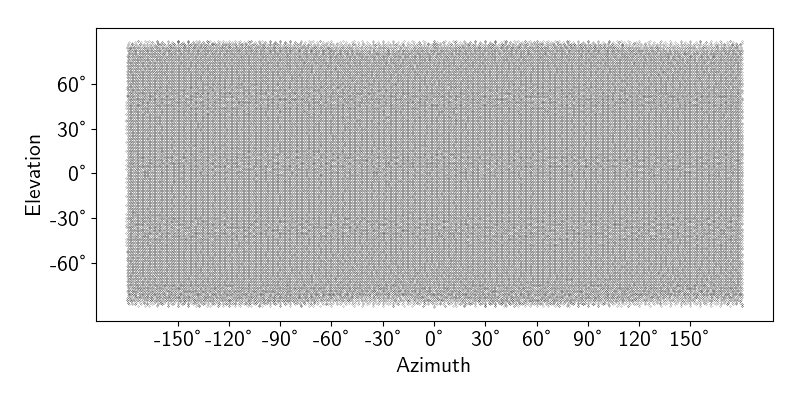
\includegraphics[width=0.7\textwidth]{Figures/res3d192k.png}
\end{subfigure}
    \caption{Figures depict from top-to-bottom SRP-PHAT angular resolution of localization with sample rate of 12kHz, 48kHz and 192kHz.}
    \label{fig:res_diff_3d}
\end{figure}
\subsubsection{Effect of change in aperture size or sample rate}
As discussed above and shown in fig. \ref{fig:res_diff}, reducing the aperture size or sample rate also reduces the angular resolution of localization, which causes a direct degradation in SRP-PHAT performance. Fig. \ref{fig:4mic1srcAper} depicts the effect of reducing sample rate or aperture size on the SRP-PHAT localization results.
\begin{figure}[H]
    \centering
    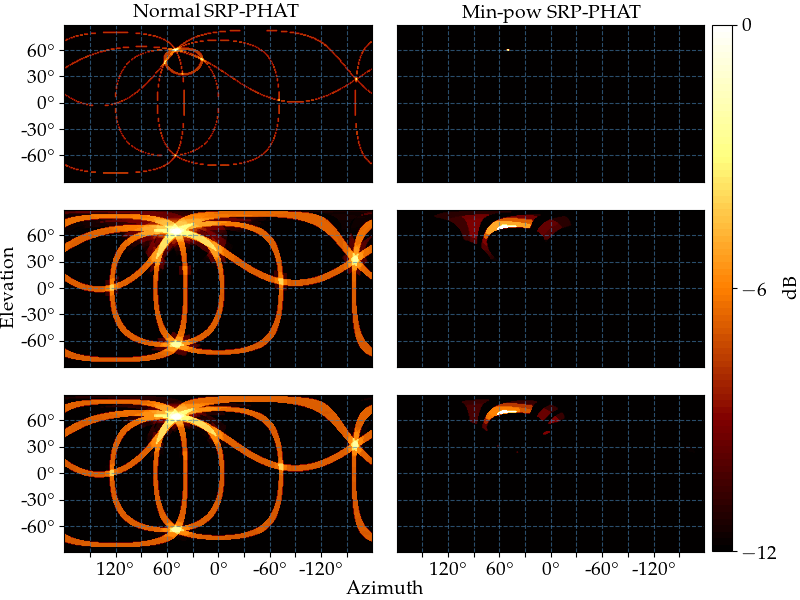
\includegraphics[width=\textwidth]{Figures/aperSampSim.png}
    \caption{Figures depict from top-to-bottom SRP-PHAT localization results with tetrahedral microphone array aperture size of 1m@48kHz, 10cm@48khz and 1m@4.8kHz.}
    \label{fig:4mic1srcAper}
\end{figure}
%\subsubsection{Effect of adding more microphones}
%It is of interest to test the scalability of the algorithm by adding more microphones. Theoretically, adding microphones should add independent pairs and thus lower the noise floor (normalized) to improve results in a low SNR scenario. 
%\begin{figure}[H]
%\begin{subfigure}[b]{0.96\textwidth}
%    \centering
%    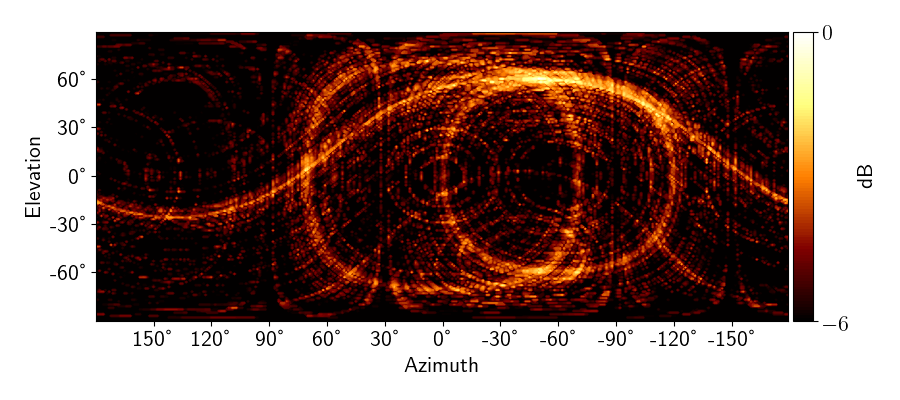
\includegraphics[width=0.8\textwidth]{Figures/Ind4mic1srcResNeg10LowDyn.png}
%\end{subfigure}
%\vskip \baselineskip
%\begin{subfigure}[b]{0.96\textwidth}
%    \centering
%    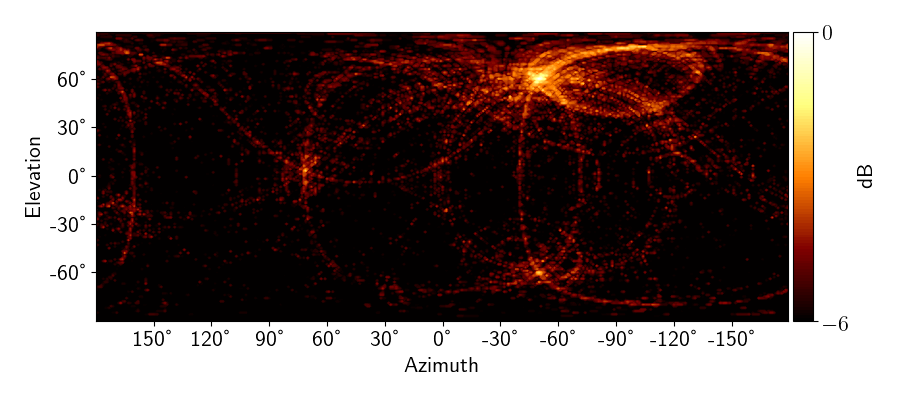
\includegraphics[width=0.8\textwidth]{Figures/Dep4mic1srcResNeg10LowDyn.png}
%\end{subfigure}
%\caption{Figures depict from SRP-PHAT localization results with SNR = -10dB, for independent microphone pairs (top), and for all  microphone pairs (bottom)}
%\label{fig:4mic1srcRedun}
%\end{figure}

\subsubsection{Effect of error in mic position}
The microphones in the array could have an error in position, due to structural errors (structural fatigue and sag, thermal expansion/ contraction or just human error). This could lead to an error in localization. Fig. \ref{fig:micErrPos} illustrates this effect. 
\begin{figure}[H]
    \centering
    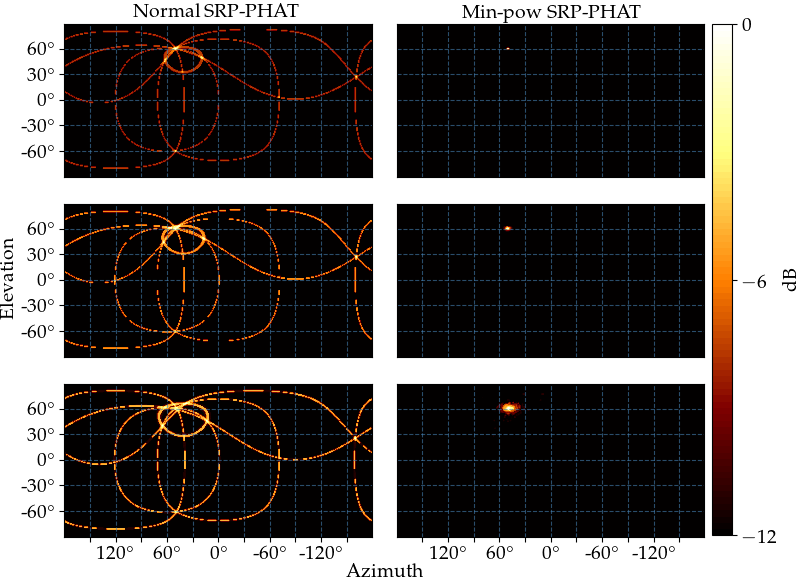
\includegraphics[width=\textwidth]{Figures/micErrPosSim.png}
    \caption{Figures depict from top-to-bottom SRP-PHAT localization results with tetrahedral microphone array with no mic error in placement (top), a 1cm placement error in 1 mic (middle), a 2cm placement error in all mics (bottom)}
    \label{fig:micErrPos}
\end{figure}

\subsubsection{Effect of error in array tilt}
\begin{figure}[H]
    \centering
    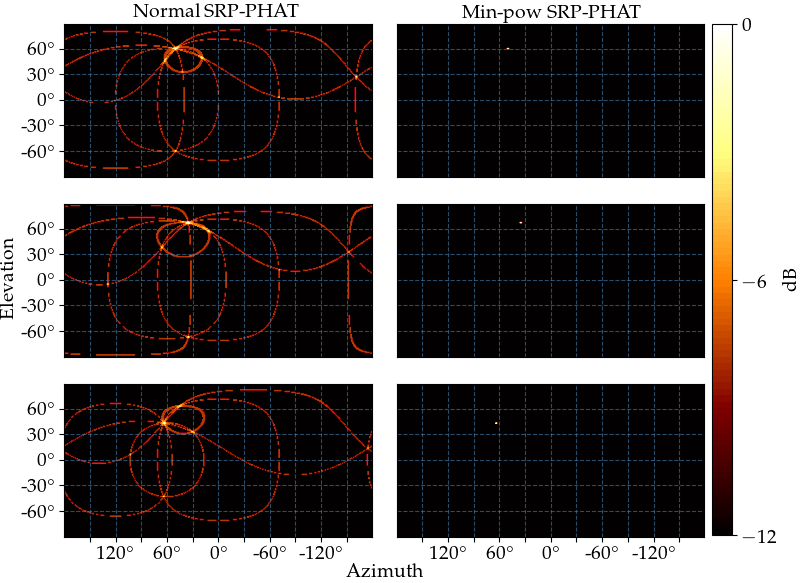
\includegraphics[width=\textwidth]{Figures/micErrTiltSim.png}
    \caption{Figures depict from top-to-bottom SRP-PHAT localization results with tetrahedral microphone array with no mic tilt error (top), a +10$\degree$ tilt  error (middle) along the x-axis and a -20$\degree$ tilt error along the x-axis (bottom)}
    \label{fig:micErrTilt}
\end{figure}
\subsubsection{Effect of audio recording length}
\begin{figure}[H]
    \centering
    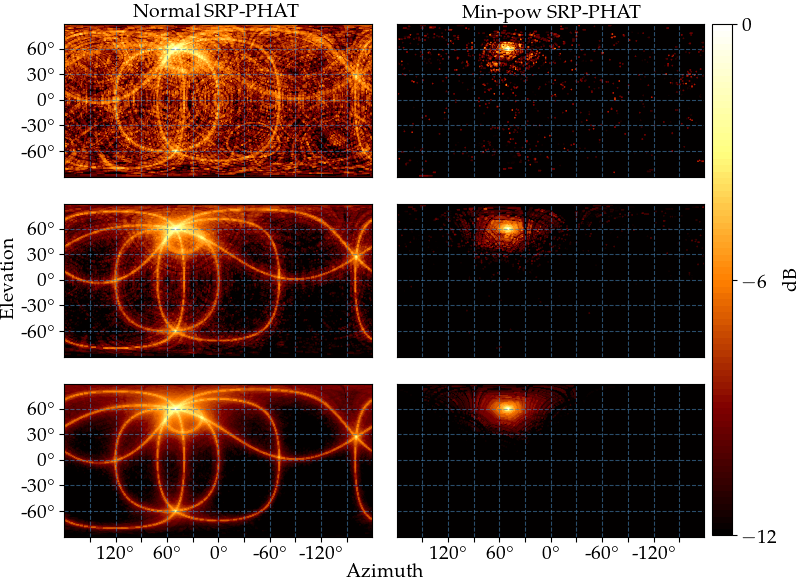
\includegraphics[width=\textwidth]{Figures/audioLenSim.png}
    \caption{Figures depict from top-to-bottom SRP-PHAT localization results with tetrahedral microphone array with recording length of 1sec  (top), 10sec (middle) and 100sec (bottom)}
    \label{fig:micErrTilt}
\end{figure}

